\section{Operator Logika}

Operator logika---disebut pula penghubung logika (logical connectives) atau operator kebenaran (truth-functional connectives)---menggabungkan proposisi menjadi proposisi majemuk \cite{levin_discrete,rosen2019}. Setiap operator mendefinisikan suatu fungsi kebenaran: nilai kebenaran proposisi majemuk ditentukan semata-mata oleh nilai kebenaran proposisi-proposisi penyusunnya. Dalam literatur, kelima operator utama sering disebut sebagai basis fungsional yang cukup untuk mengekspresikan semua fungsi kebenaran biner \cite{forallx,brilliant_truthtables}.

\begin{table}[htbp]
\centering
\small
\begin{tabular}{|c|l|l|>{\raggedright\arraybackslash}p{4.2cm}|}
\hline
\textbf{Simbol} & \textbf{Nama (ID / EN)} & \textbf{Makna} & \textbf{Benar ketika} \\
\hline
$\neg$ & Negasi / NOT & tidak, bukan & $p$ salah \\
\hline
$\wedge$ & Konjungsi / AND & dan & $p$ dan $q$ keduanya benar \\
\hline
$\vee$ & Disjungsi / OR & atau (inklusif) & Minimal satu dari $p$, $q$ benar \\
\hline
$\rightarrow$ & Implikasi / IF--THEN & jika ... maka ... & Tidak terjadi $p$ benar dan $q$ salah \\
\hline
$\leftrightarrow$ & Bikondisional / IFF & jika dan hanya jika & $p$ dan $q$ sama nilai kebenarannya \\
\hline
\end{tabular}
\caption{Ringkasan operator logika proposisional}
\label{tab:operator-logika}
\end{table}

\textbf{Negasi} ($\neg$) menyatakan ``tidak'' atau ``bukan''. Jika $p$ benar maka $\neg p$ salah, dan sebaliknya. Negasi merupakan operator uner (hanya beroperasi pada satu proposisi). Dalam bahasa alami, negasi dapat dinyatakan dengan ``tidak demikian halnya bahwa...'' atau ``adalah salah bahwa...'' \cite{copi2014}. Notasi alternatif untuk negasi meliputi $\sim p$, $\bar{p}$, atau $\lnot p$ \cite{wiki_proplogic}.

\textbf{Konjungsi} ($\wedge$) menyatakan ``dan''. Proposisi $p \wedge q$ benar hanya jika $p$ dan $q$ keduanya benar; dalam semua kasus lain, $p \wedge q$ salah. Konjungsi bersifat komutatif ($p \wedge q \equiv q \wedge p$) dan asosiatif. Notasi lain untuk konjungsi meliputi $p \cdot q$, $p \mathrel{\&} q$, atau dalam pemrograman, \texttt{AND} \cite{brilliant_truthtables,uw_boolean}.

\textbf{Disjungsi} ($\vee$) menyatakan ``atau'' dalam pengertian inklusif (inklusif OR). Proposisi $p \vee q$ benar jika minimal salah satu dari $p$ atau $q$ benar; dengan kata lain, $p \vee q$ salah hanya ketika $p$ dan $q$ keduanya salah. Perlu diperhatikan bahwa dalam logika proposisional standar, ``atau'' bersifat inklusif (``A atau B atau keduanya''), berbeda dari ``atau eksklusif'' (XOR) yang bernilai benar hanya jika tepat salah satu benar \cite{rosen2019,berkeley_logic}.

\textbf{Implikasi} ($\rightarrow$) menyatakan ``jika ... maka ...''. Proposisi $p \rightarrow q$ salah hanya jika anteseden $p$ benar dan konsekuen $q$ salah; dalam ketiga kasus lain (p salah–q benar, p salah–q salah, p benar–q benar), implikasi bernilai benar \cite{forallx}. Karakteristik ini sering membingungkan pembelajar karena secara intuitif, ketika $p$ salah, $p \rightarrow q$ tetap dianggap benar (``vacuously true''). Implikasi material dalam logika matematika memang didefinisikan demikian untuk kemudahan analisis formal \cite{brilliant_truthtables,libretexts_logic}.

\textbf{Bikondisional} ($\leftrightarrow$) menyatakan ``jika dan hanya jika'' (sering disingkat ``iff''). Proposisi $p \leftrightarrow q$ benar jika $p$ dan $q$ memiliki nilai kebenaran yang sama (keduanya benar atau keduanya salah). Bikondisional dapat dipandang sebagai konjungsi dua implikasi: $(p \rightarrow q) \wedge (q \rightarrow p)$. Notasi alternatif: $p \equiv q$ atau $p \Leftrightarrow q$ \cite{wiki_proplogic,levin_discrete}.

Selain kelima operator di atas, beberapa sistem logika mengenal operator tambahan seperti XOR (exclusive or), NAND, dan NOR. Namun, kelima operator---negasi, konjungsi, disjungsi, implikasi, dan bikondisional---sudah cukup untuk mengekspresikan seluruh ragam fungsi kebenaran dalam logika proposisional klasik \cite{rosen2019,copi2014}.

Proposisi majemuk dapat direpresentasikan sebagai pohon: simpul daun adalah proposisi atomik, simpul dalam adalah operator. Gambar~\ref{fig:pohon-proposisi} memperlihatkan pohon untuk $(p \wedge q) \rightarrow \neg r$.

\begin{figure}[htbp]
\centering
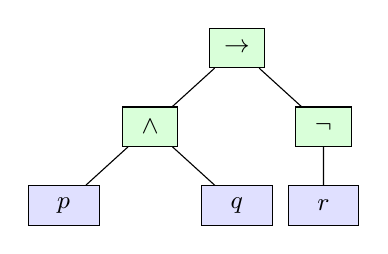
\begin{tikzpicture}[
  level distance=1cm,
  sibling distance=2.2cm,
  every node/.style={font=\small},
  atom/.style={rectangle, draw=black, fill=blue!12, minimum width=0.9cm, minimum height=0.5cm},
  op/.style={rectangle, draw=black, fill=green!15, minimum width=0.7cm, minimum height=0.5cm}
]
  \node[op] (impl) {$\rightarrow$}
    child { node[op] (and) {$\wedge$}
      child { node[atom] (p) {$p$} }
      child { node[atom] (q) {$q$} }
    }
    child { node[op] (neg) {$\neg$}
      child { node[atom] (r) {$r$} }
    };
\end{tikzpicture}
\caption{Pohon proposisi majemuk $(p \wedge q) \rightarrow \neg r$: daun = atom ($p$, $q$, $r$), simpul dalam = operator ($\wedge$, $\neg$, $\rightarrow$)}
\label{fig:pohon-proposisi}
\end{figure}

\begin{contoh}
\textbf{Terjemahan kalimat alami ke simbol logika} \cite{forallx,rosen2019}

Misalkan $p$ = ``Hari ini hujan'', $q$ = ``Saya basah''. Maka:
\begin{itemize}
  \item ``Jika hari ini hujan maka saya basah'' $\Rightarrow$ $p \rightarrow q$.
  \item ``Saya lulus jika dan hanya jika IPK $\geq 2{,}0$'': misalkan $p$ = ``Saya lulus'', $q$ = ``IPK $\geq 2{,}0$''; maka $p \leftrightarrow q$.
  \item ``Tidak hujan dan saya tidak basah'' $\Rightarrow$ $\neg p \wedge \neg q$.
\end{itemize}
\end{contoh}
